\documentclass[11pt,a4paper]{article}
\usepackage[margin=25mm]{geometry}
\usepackage[T1]{fontenc}
\usepackage{lmodern,microtype}
\usepackage{amsmath,amssymb,graphicx,booktabs,array,longtable,xcolor}
\usepackage[round,authoryear]{natbib}
\usepackage{xurl}
\usepackage[colorlinks=true,linkcolor=blue,citecolor=blue,urlcolor=blue]{hyperref}
\hypersetup{pdftitle={Instrument and Gas-Model Sensitivity of Fe II Relative-Frequency Tests in Archival Quasar Spectra},pdfauthor={Liang Wang}}
\setlength{\emergencystretch}{3em}
\graphicspath{{figures/}{../figures/}}
% Final verified numbers are entered in generated tables.

\title{Instrument and Gas-Model Sensitivity of Fe II Relative-Frequency Tests in Archival Quasar Spectra}
\author{Liang Wang\thanks{\href{mailto:wangliang.f@gmail.com}{wangliang.f@gmail.com}}}
\date{September 21, 2026}

\begin{document}
\maketitle
\begin{abstract}
Small relative shifts between absorption transitions can reflect gas structure, calibration and instrumental response as well as atomic-frequency changes. We examine these dependencies using public Fe\,II spectra. Joint fits to six ESPRESSO transitions in the $z\simeq1.1508$ absorber towards HE\,0515$-$4414 compare laboratory-frequency relations with additional relative shifts. Their conditional preference depends on pixel covariance, strong-core exclusions and gas architecture. Continuum controls measure correlated noise, while derivative projections quantify the information removed by masking. Native-pixel fits to all 17 public exposures compare the same transition in overlapping orders. A centred positive asymmetric response family retains a 2600 order contrast near $-59\,\mathrm{m\,s^{-1}}$; this does not isolate its instrumental or model origin. We also screen 36 catalogued absorbers in 32 UVES spectra, identifying six candidates under stated quality criteria. A common 2382/2374 descriptor permits an explicit cross-age identifiability analysis. Unrestricted target-specific differential offsets span the age response, while finite smooth-distortion scenarios are suppressed by the pair's small separation. At the six redshifts, normalized inverse-logarithmic schedules with powers 1, 2 and 3 have nearly indistinguishable shapes after fitting an intercept and amplitude. The contribution is a reproducible sensitivity and identifiability study. It establishes neither a calibrated fine-structure-constant variation nor a preferred cosmic-age law.
\end{abstract}

\section{Introduction}
\label{sec:introduction}
Quasar absorption spectra test laboratory transition-frequency relations in material observed at earlier cosmic epochs. Unresolved gas structure, saturation and wavelength-dependent instrumental errors can mimic differential shifts even between lines of one ion. The relevant observable is therefore a parameter of a joint spectral model whose reference transition, nuisance freedom and error convention must be stated explicitly.

\citet{Murphy2022ESPRESSO} released combined and extracted ESPRESSO spectra and modelling inputs for the exceptionally high signal-to-noise $z\simeq1.1508$ absorber towards HE\,0515$-$4414. Their multi-ion result, $\Delta\alpha/\alpha=1.3\pm1.3_{\rm stat}\pm0.4_{\rm sys}$ parts per million, is consistent with no variation. Our Fe\,II analysis examines the stability of relative line-displacement diagnostics under selected absorption and instrument assumptions. It does not replace that result or reproduce its complete uncertainty budget.

These concerns are established. \citet{WhitmoreMurphy2015} characterized relevant wavelength distortions. For the same ESPRESSO absorber, \citet{Lee2023Models} examined model construction and the treatment of a temporarily fixed constant using an ensemble more extensive than our fixed-architecture controls. \citet{Schmidt2024LSF} measured position- and slice-dependent non-Gaussian instrumental profiles, demonstrating why a Gaussian width alone is incomplete. We do not claim the first recognition of these effects.

We connect three diagnostics: matched-pixel conventional/free-shift comparisons under covariance, masking and gas-structure changes; native-exposure comparisons of the same transition in overlapping orders; and catalogue screening followed by actual-pixel checks and physical-profile fits. Available spectra, usable multiplets and calibrated frequency measurements are separate quantities. The additional contribution is to examine the identifiability of a common pair descriptor across absorbers, before interpreting any apparent age dependence.

An improved objective under extra shifts is conditional on the models and weights, without automatic calibration over component selection or instrumental uncertainty. Conversely, a baseline quadratic statistic below unity per nominal degree of freedom does not invalidate a relative preference on the same data. Both distinctions matter when formal errors are small.

The analysis is exploratory: controls follow inspection of earlier results, and archive pilot windows were chosen after profile inspection. Section~\ref{sec:methods} defines the tests; Sec.~\ref{sec:results} reports their outcomes; Sec.~\ref{sec:identifiability} examines cross-age identifiability; and Sec.~\ref{sec:discussion} describes the remaining requirements. Section~\ref{sec:prospective} outlines a prospective prediction test, detailed in Appendix~\ref{app:prediction}.

\section{Data, observables and methods}
\label{sec:methods}

\subsection{Released spectra and analysis scope}
\label{sec:data}
We use the public HE\,0515$-$4414 ESPRESSO combined spectrum, 17 extracted exposures from 2018--2020, and archived component, atomic, fitting-region and reduction inputs \citep{Murphy2022ESPRESSO}. The right-hand absorption region supplies 2931 valid pixels in six Fe\,II transitions, labelled 2260, 2344, 2374, 2382, 2586 and 2600 by approximate rest wavelength in \AA. Computations use precise archived wavelengths. Source blend exclusions particularly affect 2344 and 2586; 1608 is outside ESPRESSO coverage for this absorber.

The FITS statistical-error and expected-fluctuation arrays are kept distinct; neither supplies complete covariance. Source validity, finite values and positive errors determine usable pixels, with no new pointwise residual clipping. The principal comparison uses statistical errors. Every hypothesis pair uses identical pixels and weights.

Native S2D products are already extracted, wavelength-calibrated and sky-subtracted. Their vacuum-barycentric coordinates receive no second correction. We use \texttt{SCIDATA}, \texttt{ERRDATA} and \texttt{QUALDATA}=0, retaining separate traces and orders. Published clipping rectangles are transferred to overlapping native bins. Atmospheric intervals are shifted by exposure barycentric velocity and padded by $0.25\,\mathrm{km\,s^{-1}}$. This conservative transfer is not a full reduction replay.

UVES comparisons use SQUAD DR1 vacuum--heliocentric grids \citep{Murphy2019SQUAD}. Its 1999--2009 HE\,0515$-$4414 product records exposure shift/slope corrections, without established equivalence to a dedicated precision-analysis product. Each spectrum is fitted on its supplied grid; retrieval dates are not observing epochs.

\subsection{Relative shifts and the forward absorption model}
\label{sec:estimand}
For transition $j$, define a logarithmic velocity coordinate
\begin{equation}
 x_j=c\ln\!\left[\frac{\lambda}{\lambda_{j,\mathrm{lab}}(1+z_{
 \mathrm{ref}})}\right].
 \label{eq:velocity_coordinate}
\end{equation}
Common gas velocities remain free. Component $k$ supplies $N_k$, $v_k$ and Doppler width $b_k$, shared by all Fe\,II lines. Laboratory isotope wavelengths, damping constants and oscillator strengths use the archived \citet{MurphyBerengut2014} input. Isotope strengths already include abundances and are not weighted twice.

The conventional model fixes laboratory frequency relations and sums component and isotope optical depths before exponentiation. Its combined-spectrum prediction is
\begin{equation}
 m_{ji}=C_j(x_{ji})\left\{Z_j+(1-Z_j)
 \mathcal{P}_{ji}\!\left[L_j*\exp\!\left(-\sum_k\tau_{jk}\right)\right]\right\},
 \label{eq:forward_model}
\end{equation}
where $L_j$ is the instrumental kernel and $\mathcal{P}_{ji}$ averages over pixel $i$. The linear continuum correction $C_j$ is evaluated at the pixel centre, with the published multiplicative corrections as its baseline. The Gaussian baseline widths follow the released analysis: FWHM $2.10\,\mathrm{km\,s^{-1}}$ for 2260--2382 and $2.05\,\mathrm{km\,s^{-1}}$ for 2586 and 2600. Fixed residual levels are $Z_j=0.002$ for 2344 and 2382, $0.003$ for 2600, and zero otherwise. These levels rescale the absorption contrast as well as adding flux. The normalized transmission is convolved before pixel integration; transforming an already convolved weak-line profile by a power would not implement this model.

The 45-component $H_0$ re-optimizes 135 gas and 12 continuum parameters. $H_1$ adds shifts $\delta_j$ of the intrinsic opacity, fixing $\delta_{2374}=0$ and fitting the other five. Positive $\delta_j$ moves absorption to longer wavelength. Fixing the reference removes degeneracy with a common gas velocity.

For comparison across absorbers we retain the 2382/2374 pair, write its fitted velocity contrast as $D=\widehat\delta_{2382}$, and define
\begin{equation}
 Y_{\rm app}=\widehat\eta=-\frac{D}{c}.
 \label{eq:eta}
\end{equation}
If a fitted displacement were entirely a rest-frequency change, this would equal
\begin{equation}
 \eta=\ln\!\left[\frac{(\nu_{2382}/\nu_{2374})_{
 \mathrm{abs}}}{(\nu_{2382}/\nu_{2374})_{\mathrm{lab}}}\right].
 \label{eq:frequency_ratio}
\end{equation}
The fractional ratio change would be $e^\eta-1\simeq\eta$. Calibration, isotopes and gas modelling prevent automatically identifying the fitted descriptor with that physical change. Nor are five free shifts an $\alpha$ model, which instead predicts $\delta_j\simeq-c(K_j-K_{2374})\Delta\alpha/\alpha$ along one direction specified by atomic sensitivities $K_j=\partial\ln\nu_j/\partial\ln\alpha$.

\subsection{Quadratic objectives, covariance and fixed core masks}
\label{sec:covariance}
For data vector $f$, fixed covariance $\Sigma$ and model $m(\theta)$, the working objective is
\begin{equation}
 Q(\theta)=[m(\theta)-f]^{\mathsf T}\Sigma^{-1}[m(\theta)-f].
 \label{eq:objective}
\end{equation}
Under fixed Gaussian errors this is the usual $\chi^2$. We report $\Delta Q=Q_0-Q_1$ within a matched pair, equivalent to the historical output label $\Delta\chi^2$. Different masks or weights do not define one common likelihood-ratio statistic.

Correlation controls place 36 candidate intervals at fixed offsets, excluding all authors' fitting windows and duplicate/invalid pixels. Recorded retention, median-flux and broad-feature criteria leave 25 disjoint intervals containing 13,750 pixels. After linear-continuum removal without pixel clipping, we correlate residuals normalized by supplied errors and bootstrap whole intervals 10,000 times. Alternative detrending and thresholds are saved. These controls were designed after data inspection.

For the nonlinear covariance test we use the fixed tapered correlation matrix
\begin{equation}
 R_{ij}=\begin{cases}
 \widehat\rho_{\ell}(1-\ell/11),&\ell=|n_i-n_j|\leq10,\\
 0,&\ell>10,
 \end{cases}
 \qquad \Sigma_{ij}=s_iR_{ij}s_j,
 \label{eq:tapered_covariance}
\end{equation}
Original indices $n_i$ preserve separations across masked gaps; widely separated lines are treated independently. Residuals and derivatives receive the same Cholesky whitening. The continuum variance amplitude is not transferred; a uniform rescaling would leave optima unchanged. Transfer of the correlation shape to deep absorption remains conditional.

Frozen masks use the original diagonal-noise $H_0$ prediction for 2382 and 2600: flux below 0.1, or below 0.3 with three-pixel ($1.2\,\mathrm{km\,s^{-1}}$) padding. We test masking and covariance separately and together. To quantify information loss, local derivatives at that fixed $H_0$ give both strong lines a $100\,\mathrm{m\,s^{-1}}$ shift, with other relative shifts zero; gas/continuum directions are projected out under GLS weights. This ignores bounds and characterizes one direction, not five-shift marginal information or a detection.

\subsection{Gas structure, bounds and numerical endpoints}
\label{sec:optimization}
The principal gas search allows velocities within $\pm2\,\mathrm{km\,s^{-1}}$ and column densities within $\pm2$ dex of the published initialization, with $7\leq\log_{10}(N/\mathrm{cm^{-2}})\leq17$ and $0.15\leq b\leq30\,\mathrm{km\,s^{-1}}$. Continuum coefficients lie within $\pm0.03$, with the slope multiplying a centred velocity divided by $100\,\mathrm{km\,s^{-1}}$. Relative shifts lie within $\pm0.5\,\mathrm{km\,s^{-1}}$. Wider bounds, opacity/zero-level freedom, modified Gaussian widths and transition exclusions are separately recorded controls, not measured calibration priors.

A fixed alternative architecture joins adjacent published component centres separated by less than $1.025\,\mathrm{km\,s^{-1}}$ into connected groups, producing 40 components. Each merged initialization preserves total column density, its weighted centre and the Doppler-core second moment:
\begin{equation}
 v_g=\sum_k w_kv_k,\qquad
 b_g^2=\sum_k w_k\{b_k^2+2(v_k-v_g)^2\},\qquad
 w_k=\frac{N_k}{\sum_{k\in g}N_k}.
\end{equation}
This is not preservation of a finite variance of the full Voigt profile. Nor does the separation rule prove that sub-resolution structure is unmeasurable. Bounds of the same widths are centred on the merged initialization, so this is a combined architecture-and-bounds sensitivity test, not a nested selection of the true cloud count.

Constrained fits retain starts, opposite-hypothesis starts, continuations and unsuccessful endpoints. Stopping flags, first-order stationarity and global optimality are distinguished; UVES continuations include explicit bound-gradient checks. Independent implementations replay atomic normalization, residuals, derivatives, covariance and saved objectives, and refine pixel quadrature. These verify numerical consistency, not physical adequacy or significance.

\subsection{Native exposures and centred response controls}
\label{sec:orders}
Native fits use a gas template fixed from the combined-spectrum $H_0$, exposure line velocities, and per-row continuum amplitude/slope and additive zero. Relative shifts subtract 2374 while retaining its shared-reference covariance. The same estimator is applied to the combined spectrum; it differs from re-optimizing all gas parameters.

Overlapping orders provide the lower-index minus upper-index velocity of the same transition, cancelling 2374 entirely. Disjoint samples can still share extraction errors. We test leave-one-exposure stability, separate traces, and date, barycentric-velocity, signal-to-noise and detector-position predictors. Pixel phase is the fractional interpolated position of a fixed velocity reference, treated circularly. All regressions are reported; correlated predictors and post-inspection design preclude causal or multiplicity-calibrated interpretation.

A further matched analysis fits each transition jointly across exposures. It compares Gaussian kernels with a positive, normalized asymmetric family. For order $o$ the latter is
\begin{equation}
 L_o(u)=0.8\,\phi_s(u+0.2d_o)+0.2\,\phi_s(u-0.8d_o),
 \label{eq:mixture_lsf}
\end{equation}
where $\phi_s$ is a zero-mean Gaussian of standard deviation $s$, $d_o=1.2\,\mathrm{km\,s^{-1}}\,\mathrm{cbrt}(a_o)$, $-1\leq a_o\leq1$, and
\begin{equation}
 s^2=(w_o/2.354820045)^2-0.16d_o^2.
\end{equation}
Here $1.6\leq w_o\leq2.6\,\mathrm{km\,s^{-1}}$ is a Gaussian-equivalent variance width, not literal FWHM. The kernel centroid is zero at every asymmetry. Each order shares one width and shape across all 17 exposures and both traces: a strong sensitivity assumption given known slice dependence, not a calibrated response. Each family is fitted with/without a common order offset and with exposure velocities. Per-row continuum/zero coefficients are profiled by weighted linear least squares, retaining residual-dependent derivative terms.

A transfer test freezes response parameters fitted to nine 2018 exposures when evaluating eight later exposures, refitting velocities and continua. The photon subsets are disjoint but the combined-data gas template is shared. This restricted shape family is a stress test, not an independent LSF calibration.

\subsection{Archive screening and additional absorbers}
\label{sec:archive_methods}
We screen 155 catalogued damped Ly$\alpha$ absorbers in SQUAD for nine Fe\,II lines: full $\pm250\,\mathrm{km\,s^{-1}}$ coverage, forest avoidance with a $3000\,\mathrm{km\,s^{-1}}$ margin, atmospheric bands and catalogue CNR. Broader water-band exclusions are an explicit amendment. These approximate metadata gates do not certify clean observed lines.

All 32 spectra containing 36 initial candidates are retrieved. Native-pixel validity, noise, absorption strength, three-line common structure and an unsaturated weaker-line candidate define readiness. Interpolation used for screening does not produce independent significance bins. Six systems pass, with residual edge/blend/calibration warnings retained. The targeted DLA subset does not exhaust SQUAD, and absorbers sharing a sightline share calibration.

Profile pilots use common gas components, consistent atomic data and per-line continuum, zero and Gaussian-width freedom. Windows follow profile inspection; pixels are not residual-clipped. Stated component counts and multiple starts feed an exploratory diagonal-error $H_0$ AICc selection. Both error arrays are compared for the first two pilots; the remaining four use expected-fluctuation errors directly. Common-pair profiles fix $D$ while refitting gas, instrumental and other relative-shift parameters. Thus a $D=0$ profile point is not the full laboratory-frequency $H_0$. Lower profile endpoints seed renewed matched fits; inadequate models and boundary solutions remain visible.

\subsection{A common descriptor and cosmic-age identifiability}
\label{sec:age_methods}
Section~\ref{sec:identifiability} defines a fixed illustrative age coordinate and normalized candidate schedules $G_p(z)$ (Eq.~\ref{eq:normalized_age}), with $G_p(0)=0$ and $G_p(3)=1$. These are not cosmological fits. Function shapes are compared after fitting an intercept and amplitude, independently of any measured signal.

For a velocity descriptor $D_a=-c\widehat\eta_a$ per absorber, consider
\begin{equation}
 D_a=b+A G_p(z_a)+d_a+\epsilon_a.
 \label{eq:age_nuisance}
\end{equation}
The amplitude $A$ is a velocity contrast in $\mathrm{m\,s^{-1}}$, not $\Delta\alpha/\alpha$. The absorber-specific $d_a$ describes a \emph{differential} calibration/model offset; a common log-wavelength zero point cancels. Unrestricted $d_a$ absorb $A\mapsto A+q$ through $d_a\mapsto d_a-qG_p(z_a)$. Rank and nuisance projections test this exact degeneracy. Finite nuisance constraints restore conditional information and must be distinguished from unrestricted coefficients; forecasts suppressing these terms are not independently calibrated physical bounds.

\section{Results}
\label{sec:results}

\subsection{The reference spectrum and the meaning of a free-shift improvement}

In the six-transition ESPRESSO reference fit, the restricted conventional model has 147 parameters and the alternative has 152. Both use the same 2931 retained pixels. The selected diagonal-error endpoints give $Q_0=2305.49$ and $Q_1=2253.78$, an improvement of $51.71$ for five relative shifts. The 2382 and 2600 shifts are approximately $-118$ and $-109\,\mathrm{m\,s^{-1}}$ relative to 2374. Figure~\ref{fig:reference_profiles} shows the actual profiles and residuals. Several nuisance parameters lie near their bounds, and different starts find different local solutions. The improvement therefore establishes a conditional preference within this particular comparison; it is not assigned a discovery significance or interpreted as a measurement of $\Delta\alpha/\alpha$.

The alternative supplied expected-fluctuation error array increases the diagonal-error improvement to $67.92$, with $Q_0=2801.71$ and $Q_1=2733.79$. Thus the recorded controls do not uniformly weaken the preference. This noise-amplitude change is distinct from the continuum-derived correlation-shape test below. The complete saved control grid includes both stronger and weaker conditional improvements.

\begin{figure}[htbp]
\centering
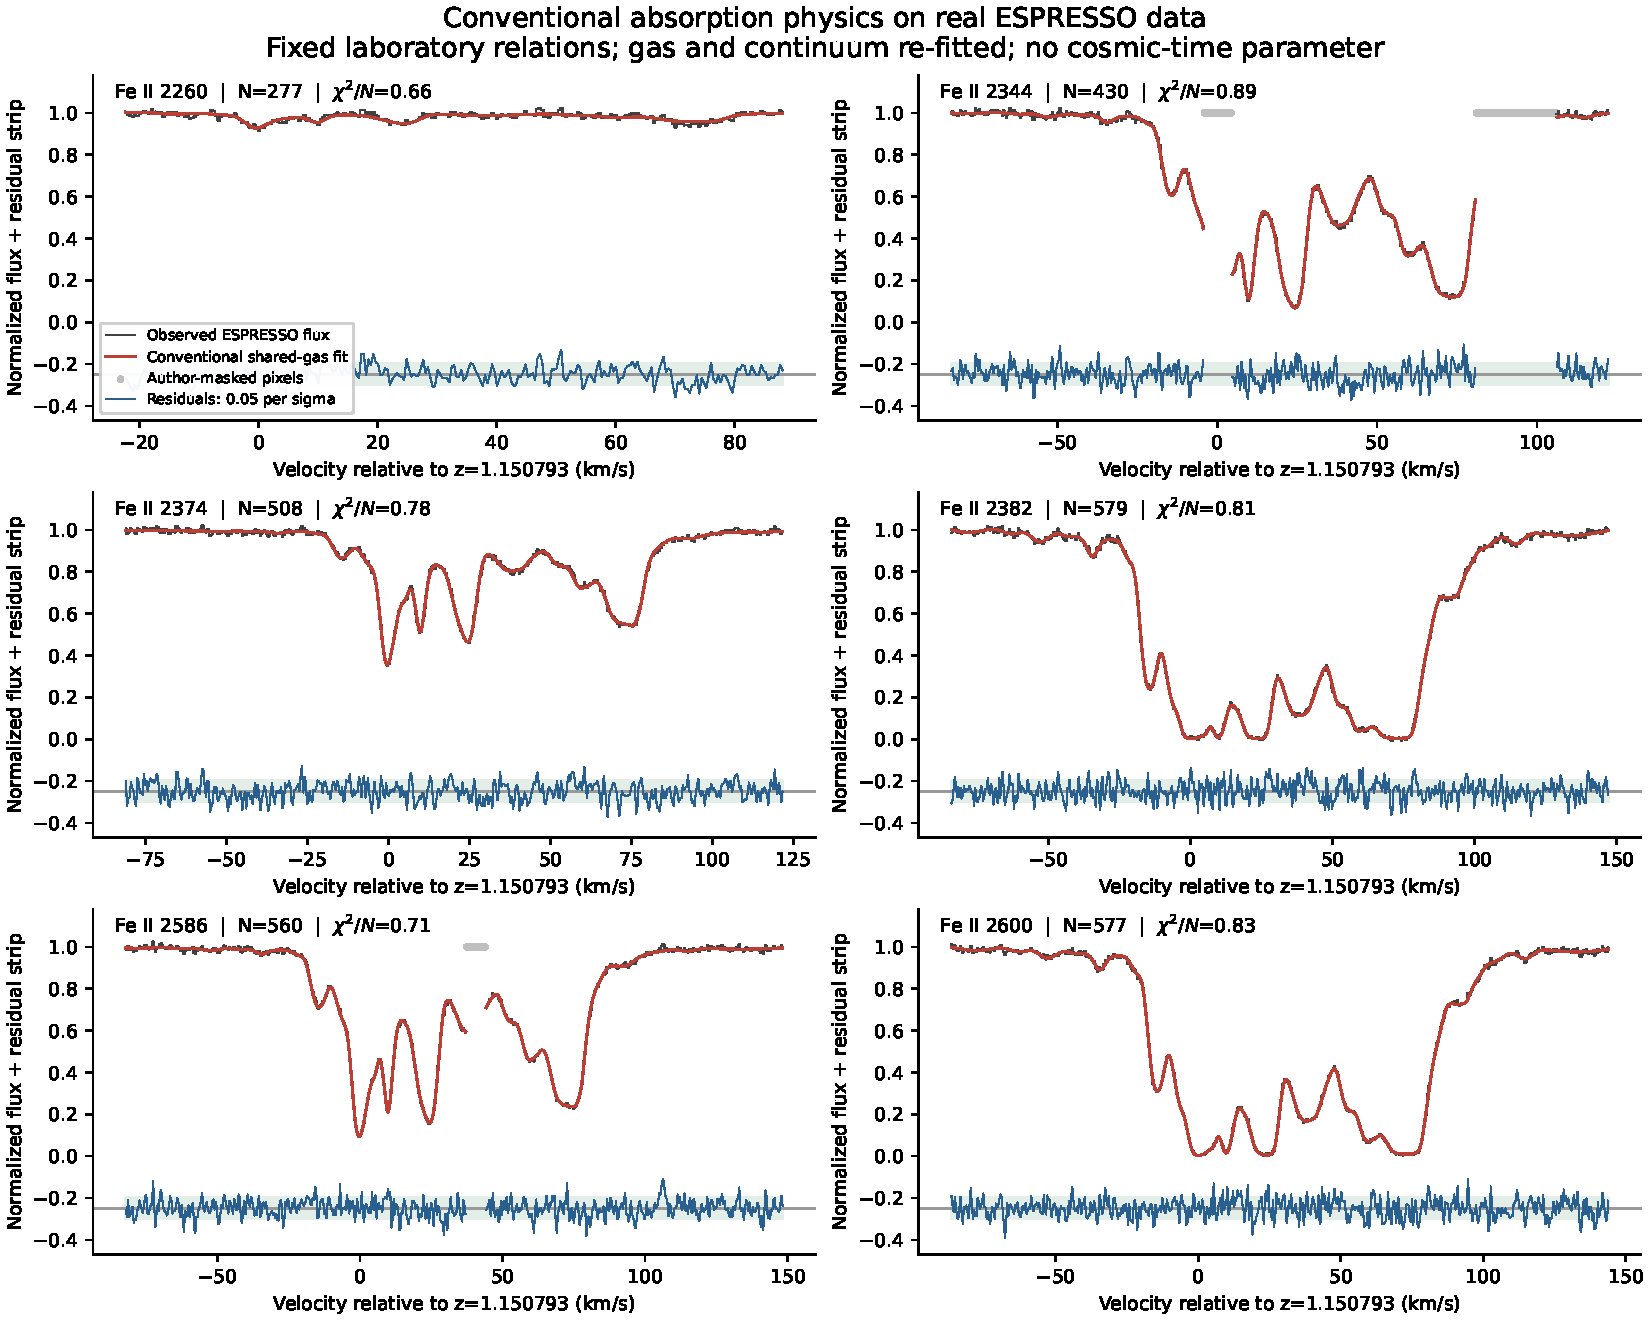
\includegraphics[width=.94\textwidth,height=.68\textheight,keepaspectratio]{espresso_conventional_null.pdf}
\caption{The six observed Fe\,II transitions in the reference ESPRESSO interval, with shared-gas fits and standardized residuals. The conventional and free-relative-shift models have the same gas and continuum freedoms. A better fit after adding shifts is a diagnostic of the specified model, not an identification of the physical origin of the discrepancy.}
\label{fig:reference_profiles}
\end{figure}

\subsection{Correlated noise, core exclusions and retained information}

Twenty-five non-overlapping continuum intervals contain 13,750 pixels. After local continuum removal, their lag-one correlation is $0.3726$. We use the measured correlation shape with a finite taper, retaining the supplied error amplitude. This is a covariance model transferred from continuum diagnostics, not a measured full covariance for the absorption spectrum. The generalized least-squares comparison reduces the five-shift improvement to $29.24$. The nonlinear fit re-optimizes gas and continuum parameters under the changed weights; it is not a rescaling of the diagonal-error result.

The joint controls apply the frozen strong-line exclusions and the same tapered correlation model simultaneously. The milder mask leaves 2692 pixels and gives an improvement of $23.69$; the padded wider mask leaves 2473 pixels and gives $6.70$. Table~\ref{tab:control_comparisons} lists within-row comparisons. The relevant hypotheses use identical pixels and covariance within each row, whereas objective differences across rows do not have a common likelihood-ratio interpretation.

\begin{table}[htbp]
\centering
\caption{Conditional reference-spectrum comparisons. $k_0$ counts conventional-model parameters; each alternative adds five shifts. GLS retains the supplied variance amplitude. All rows describe selected bounded local endpoints, with no global-optimum certification.}
\label{tab:control_comparisons}
\small
\begin{tabular}{lrrrr}
\toprule
Selection and gas architecture & Pixels & $k_0$ & $Q_0$ & $\Delta Q$ \\
\midrule
Statistical errors, diagonal, 45 components & 2931 & 147 & 2305.49 & 51.71 \\
Expected fluctuations, diagonal, 45 components & 2931 & 147 & 2801.71 & 67.92 \\
Full pixels, GLS, 45 components & 2931 & 147 & 2231.33 & 29.24 \\
Joint $F<0.1$ mask + GLS & 2692 & 147 & 1931.90 & 23.69 \\
Joint padded $F<0.3$ mask + GLS & 2473 & 147 & 1684.36 & 6.70 \\
Full pixels, GLS, 40 components & 2931 & 132 & 2255.16 & 18.87 \\
\bottomrule
\end{tabular}

\end{table}

Masking changes both model sensitivity and the available information. At the same fixed diagonal-noise conventional endpoint, we project the five shift derivatives against the gas and continuum derivatives under each GLS selection. For the specified direction in which 2382 and 2600 each move by $100\,\mathrm{m\,s^{-1}}$ and the other three shifts remain zero, the milder and wider masks retain $70.5\%$ and $16.0\%$ of the unmasked local information (Fig.~\ref{fig:core_information}). The direction was chosen to illustrate the previously observed strong-line pattern; it is not a prediction independent of these data. The calculation uses an unconstrained tangent space despite active parameter bounds. It follows that a smaller improvement after core removal cannot by itself establish that saturation caused the original shifts. Conversely, this calculation does not establish that information loss accounts for the full reduction.

\begin{figure}[htbp]
\centering
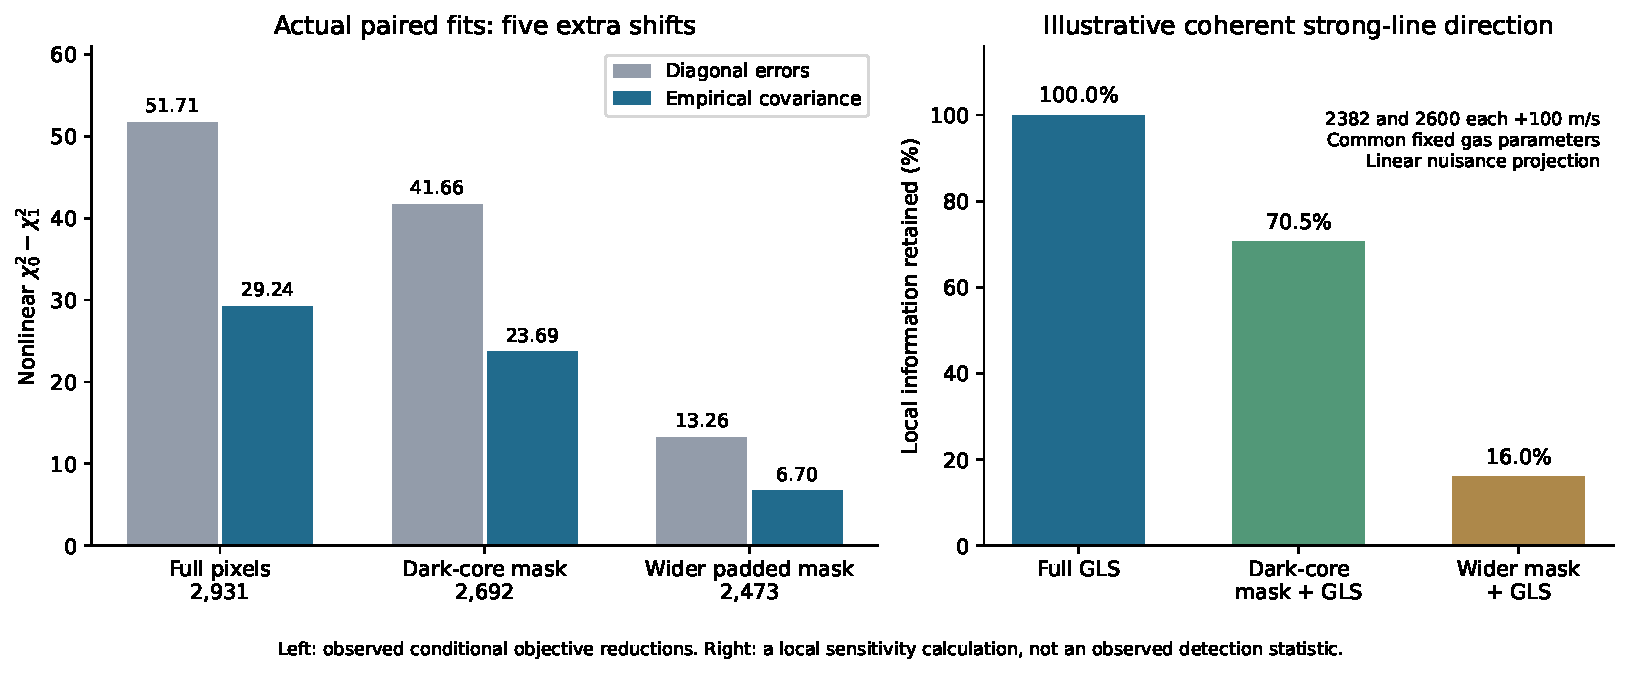
\includegraphics[width=.98\textwidth]{joint_controls_information.pdf}
\caption{Actual nonlinear objective improvements (left) and a separate local sensitivity calculation (right). The latter describes one specified coherent strong-line direction after projection over common nuisance parameters, not the marginal information for five free shifts. Diagonal and GLS fits within each mask are actual re-fits; different masks retain different information.}
\label{fig:core_information}
\end{figure}

\subsection{Gas architecture and optimization dependence}

The fixed merging rule yields 40 components from the 45 published starting components. On the full set of 2931 pixels, the 132-parameter conventional GLS model gives $Q_0=2255.16$ and the 137-parameter alternative gives $Q_1=2236.29$, an improvement of $18.87$. The 2382 and 2600 shifts become approximately $-89$ and $-80\,\mathrm{m\,s^{-1}}$, each changing by about $22\,\mathrm{m\,s^{-1}}$ from the 45-component GLS values. Two alternative-model starts terminate at objectives differing by $12.95$. Thus architecture and initialization affect the result even though this particular reduced architecture does not remove the conditional shift preference. Because the merged starting centres also define the shifted parameter-bound centres, this is an architecture-and-bounds sensitivity test, not a nested determination of the correct number of gas clouds.

The independent UVES photons from the same absorber provide an additional, explicitly limited check. Three Fe\,II lines contain 511 usable pixels. Using the recommended expected-fluctuation errors, we continue fits with Gaussian-width scales bounded by $[0.65,1.25]$ and $[0.5,1.4]$ times the catalogue value. Four 1800-evaluation continuations and one 400-evaluation conventional cross-start all reach their evaluation caps and fail the specified first-order stationarity criteria. The lowest saved conventional parameter vector is feasible in both domains. Relative to that vector, the finite objective reductions are $9.75$ and $10.08$ for two shifts; widening the instrumental-width bounds changes the strong-line offsets by only $4$--$5\,\mathrm{m\,s^{-1}}$. These nonstationary endpoint differences receive no calibrated significance. The archived product records wavelength shift and slope corrections, whose equivalence to a dedicated precision-analysis product has not been established. Independent photons therefore do not supply an independent model or a completed physical confirmation.

\subsection{Native-exposure and same-transition order tests}
\label{sec:order_results}
The fixed-template estimator applied to the 17 individual exposures gives pooled 2382 and 2600 shifts relative to 2374 of $-41.9\pm16.4$ and $-45.5\pm15.0\,\mathrm{m\,s^{-1}}$. Applying the same estimator to the combined spectrum gives $-42.8$ and $-39.6\,\mathrm{m\,s^{-1}}$. These are compatible representations of the same observations, not independent confirmations. They are also different estimators from the joint fits in which all gas parameters are re-optimized. The original exposure analysis finds no clear excess heterogeneity or difference between the nine 2018 and eight later exposures under its conditional covariance model.

The same-transition comparison removes the atomic reference entirely. In the initial per-exposure calculation, the lower-index minus upper-index order contrast is $-60.25\pm16.72\,\mathrm{m\,s^{-1}}$ for 2600, compared with $-10.53\pm21.87\,\mathrm{m\,s^{-1}}$ for 2382. The two traces separately retain the 2600 pattern, and deleting any single exposure gives means between approximately $-70.1$ and $-52.0\,\mathrm{m\,s^{-1}}$. The diagnostic is therefore not dominated by one exposure or one trace. The barycentric velocity and detector position are nearly collinear in these observations, preventing their simple regressions from locating the mechanism.

We next fit all exposures jointly with the Gaussian and centred positive-mixture response families defined in Sec.~\ref{sec:methods}. Each family has matched comparisons with and without a single order-contrast parameter. This jointly shared response estimator is slightly different from independently fitting each exposure. The completed comparisons are shown in Table~\ref{tab:order_models} and Fig.~\ref{fig:order_models}.

\begin{table}[htbp]
\centering
\caption{Native-pixel order-response controls. The order contrast is the lower-index minus higher-index order velocity for the same transition, distinct from the cross-transition descriptor $D$. G denotes the Gaussian response; A denotes the specified positive, zero-centroid asymmetric family. Subscripts indicate whether a free order contrast is added. Errors are local, conditional on the fixed gas template and diagonal extraction errors. $\Delta Q$ compares models within the indicated response family, not different transitions.}
\label{tab:order_models}
\small
\begin{tabular}{llrrr}
\toprule
Transition & Response & $Q$ & Order contrast ($\mathrm{m\,s^{-1}}$) & $\Delta Q$ \\
\midrule
2600 & G$_0$ & 41636.411 & 0 (fixed) & --- \\
2600 & G$_1$ & 41622.198 & $-62.75\pm16.66$ & 14.212 \\
2600 & A$_0$ & 41630.900 & 0 (fixed) & --- \\
2600 & A$_1$ & 41620.042 & $-58.64\pm18.65$ & 10.858 \\
2382 & G$_0$ & 39994.136 & 0 (fixed) & --- \\
2382 & G$_1$ & 39993.889 & $-11.03\pm22.18$ & 0.247 \\
2382 & A$_0$ & 39994.062 & 0 (fixed) & --- \\
2382 & A$_1$ & 39993.787 & $-13.48\pm26.35$ & 0.275 \\
\bottomrule
\end{tabular}
\end{table}

The specified asymmetric family does not remove the 2600 contrast. Relative to G$_1$, two shape parameters reduce $Q$ by only 2.16. Forcing a zero order contrast in A$_0$ drives one shape parameter to its bound. The asymmetric fit has nominal $Q/(N-k)\simeq1.34$ for 2600 and 1.29 for 2382, so even the extended response does not supply an adequate complete noise-and-profile description. Conditional objective profiles explicitly re-optimize the remaining parameters at 13 order offsets from $-120$ to $+120\,\mathrm{m\,s^{-1}}$. They confirm the local displacement preference while exposing shape boundaries; they do not supply a calibrated discovery probability. The shape parameterization is not generally twice continuously differentiable at its Gaussian limit, providing another reason to avoid an automatic Wilks interpretation.

\begin{figure}[htbp]
\centering
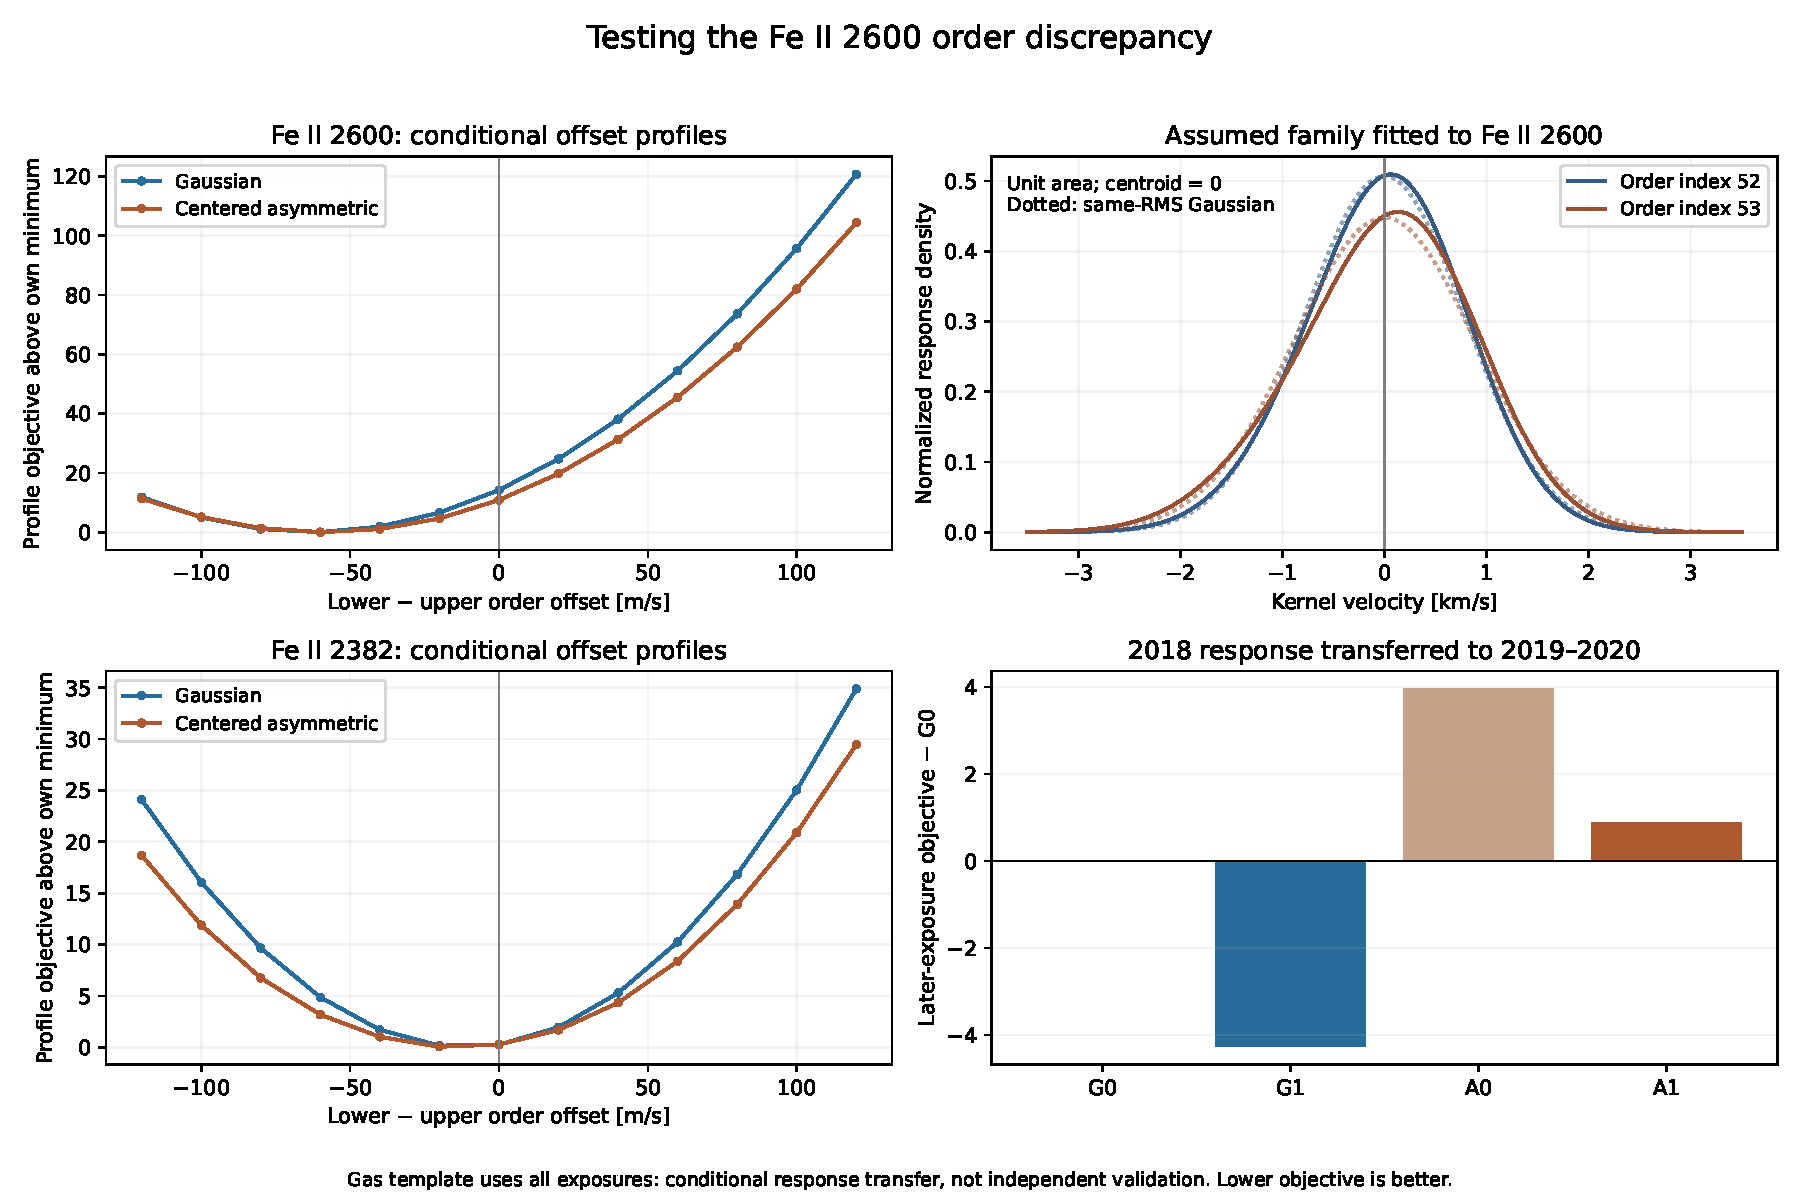
\includegraphics[width=.99\textwidth]{../experiments/highz_feasibility_2026-09-20/results/order_response/order_response_models.pdf}
\caption{Tests of the specified centred response family using actual native pixels. The order-contrast profiles re-optimize nuisance parameters at fixed contrast. The response-family illustration does not represent an independently measured LSF. The later-exposure comparison transfers response parameters learned from 2018, while the gas template remains shared with the full data set; it is therefore a conditional transfer diagnostic.}
\label{fig:order_models}
\end{figure}

In that transfer diagnostic, the Gaussian-plus-contrast model improves the later-exposure objective by 4.27 relative to the Gaussian zero-contrast model. The asymmetric-plus-contrast model is worse than Gaussian-plus-contrast by 5.15. This does not establish a transferable benefit from the extra shape parameters. An instrumental response that genuinely changes across epochs remains possible, and the shared combined-spectrum gas template prevents a fully independent predictive interpretation.

The orders also have different sampling, masks and signal-to-noise weights. A further mask control retains a native pixel only when its entire wavelength bin is covered by the other order's originally valid bins; selection uses wavelength geometry and existing quality masks, not new residual clipping. It retains 62,154 of 62,404 relevant pixels. The resulting 2600 contrast is $-58.65\pm16.75\,\mathrm{m\,s^{-1}}$, and the 2382 contrast is $-15.45\pm21.98\,\mathrm{m\,s^{-1}}$. Missing coverage alone, under this particular control, does not remove the pattern. Sampling and weighting still differ, so a shared imperfect gas template could produce different apparent velocities without a pure calibration offset.

Independent calibration remains unresolved. The released science headers identify the same \texttt{espdr/2.2.3}, SINGLEHR, $2\times1$ mode and LFC/FP wavelength products. For two representative science frames, current default archive master associations instead return THAR/FP wavelength products. Their association status does not establish reproduction of the released LFC solution. We locate historical raw LFC candidates and preserve their headers and association trees, but the checked public links do not yield uniquely matched historical LFC masters or independently measured response kernels. The 2024 response study used 2023 calibration data \citep{Schmidt2024LSF}; its method motivates this investigation, while its measured kernels cannot simply be assigned to the 2018--2020 science exposures. The bounded controls therefore locate a robust conditional order inconsistency without identifying its unique cause or measuring an intrinsic atomic change.


\subsection{The complete screened absorber sample}
\label{sec:archive_results}
The catalogue screen initially retains 36 absorbers in 32 spectra. Extending the atmospheric exclusion to broad water bands leaves seven metadata candidates; actual-pixel inspection leaves six multiplet candidates. All six are retained in the physical-model accounting in Table~\ref{tab:archive_six}, including models that remain inadequate. These are selected DLA sightlines, not a complete or statistically representative sample of metal absorbers.

For the four newly modelled candidates, an exploratory adequacy gate requires $Q_0/(N-k_0)\leq1.5$, every line's $Q/N_{\rm line}\leq1.8$, and successful optimizer termination. The thresholds are working diagnostics under the stated diagonal errors, not calibrated goodness-of-fit probabilities. Component grids, windows and visible contamination warnings were recorded before the new relative-shift fits, with documented null-model grid extensions. Because an $H_0$ gate could also reject a genuinely shifted system, we additionally perform bounded free-shift and crossed-null diagnostics for both gate failures on their unchanged primary pixels. They remain inadequate, and we do not promote them to precision measurements or use the gate to infer population-level constancy.

\begin{table}[htbp]
\centering
\caption{Latest matched conventional/free-shift comparisons for all six archive candidates. $n_g$ is the shared gas-component count and $k_\delta$ the number of additional shifts. Values use native pixels and diagonal expected-fluctuation errors. ``Conditional'' permits a model-specific displacement diagnostic, not a calibrated atomic-frequency measurement. ``Inadequate'' retains the post-screen diagnostic comparison on the original primary data. All pairs retain model and optimization limitations described in the text.}
\label{tab:archive_six}
\small
\begingroup
\setlength{\tabcolsep}{4pt}
\begin{tabular}{lrrrrrl}
\toprule
Target ($z$) & Pixels & $n_g$ & $Q_0$ & $\Delta Q$ & $k_\delta$ & Status \\
\midrule
J232128$-$105122 (1.629) & 130 & 3 & 75.16 & 6.16 & 4 & Conditional \\
J225719$-$100104 (1.836) & 504 & 30 & 421.25 & 13.53 & 2 & Conditional \\
J053007$-$250329 (2.141) & 480 & 16 & 482.30 & 4.18 & 3 & Conditional \\
J233156$-$090802 (2.143) & 1176 & 26 & 1672.84 & 5.54 & 2 & Inadequate \\
J004131$-$493611 (2.248) & 138 & 6 & 95.23 & 7.97 & 2 & Conditional \\
J064326$-$504112 (2.659) & 436 & 16 & 532.23 & 4.64 & 3 & Inadequate \\
\bottomrule
\end{tabular}
\endgroup

\end{table}

The initial two pilots now have actual nuisance-refitted profiles for $D=v_{2382}-v_{2374}$ (Fig.~\ref{fig:archive_pair}). For J232128$-$105122, the latest matched full-model comparison gives $Q_0=75.1589$, $Q_1=68.9988$ and $\Delta Q=6.1600$ for four added shifts. Its $D=-339.97\,\mathrm{m\,s^{-1}}$ has unconstrained local tangent error $179.58\,\mathrm{m\,s^{-1}}$; the connected profile has linearly interpolated $\Delta Q=1$ crossings between optimized grid points at $[-495.18,-187.88]\,\mathrm{m\,s^{-1}}$. Several zero-level parameters are bound-active. Neither the local error nor the profile contour includes calibration or gas-architecture uncertainty.

J004131$-$493611 illustrates why a stopped optimizer is not a certified solution. Profiling discovered a substantially lower nuisance basin than the earlier pair $(Q_0,Q_1)=(110.0357,104.5341)$. Restarting both full hypotheses fairly gives $(95.2285,87.2549)$, hence $\Delta Q=7.9735$ for two shifts. The revised $D=-120.11\,\mathrm{m\,s^{-1}}$ has local tangent error $399.41\,\mathrm{m\,s^{-1}}$, whereas the bounded connected $\Delta Q=1$ contour, linearly interpolated between optimized grid points, is $[-264.86,+39.96]\,\mathrm{m\,s^{-1}}$. Active gas-width, response-width and zero-level bounds may contribute to this discrepancy; nonlinearity and residual curvature have not been separately isolated. These are conditional objective contours, not coverage-calibrated confidence intervals. Fixing $D=0$ still lets 1608 move and therefore does not recover the full $H_0$.

\begin{figure}[htbp]
\centering
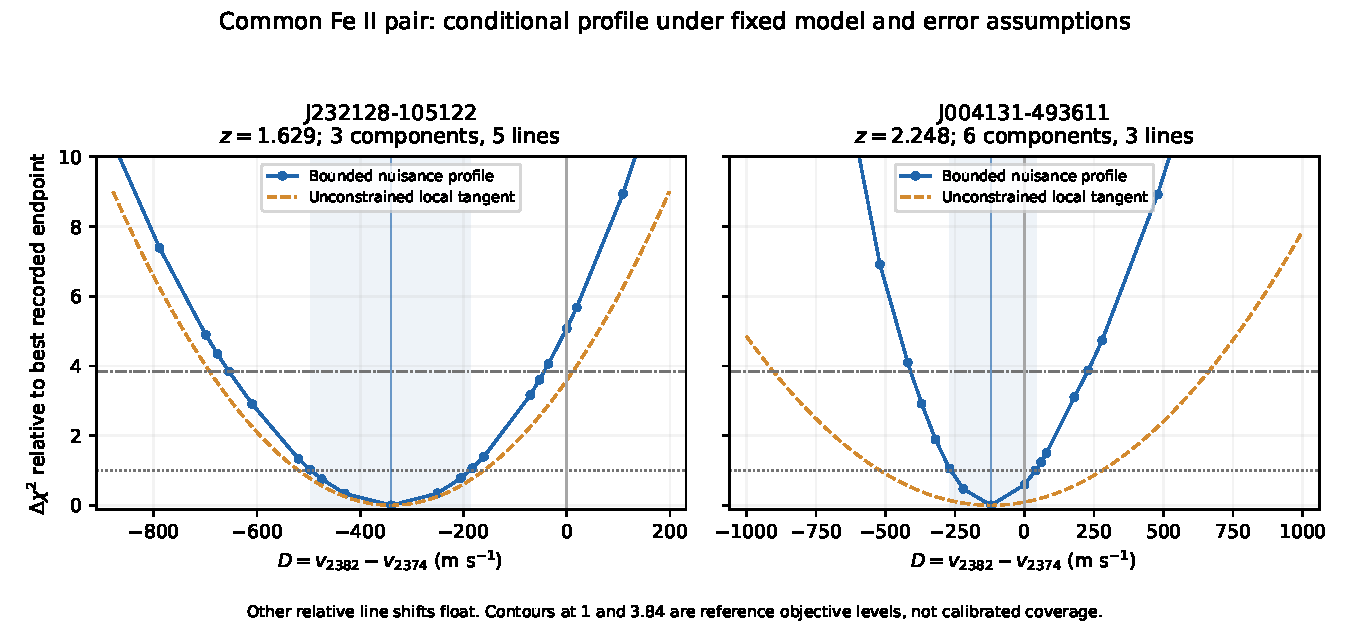
\includegraphics[width=.95\textwidth]{../experiments/highz_feasibility_2026-09-20/results/common_pair/common_pair_profiles.pdf}
\caption{Actual conditional profiles of the common 2382/2374 descriptor in the two initial pilots. Gas and other nuisance parameters, including the other relative line shifts, are refitted. Only endpoints in the final selected nuisance basins are connected; earlier inferior endpoints remain in the archive. Horizontal objective levels are descriptive. They do not calibrate systematic uncertainties, component selection or disconnected minima.}
\label{fig:archive_pair}
\end{figure}

The selected tested architecture for J053007$-$250329 has 16 gas components for four regions, including weak 1611, with 480 unique pixels. The matched comparison gives $\Delta Q=4.1760$ for three shifts. At this fixed architecture, $D=+268.78\pm130.09\,\mathrm{m\,s^{-1}}$ is a local conditional diagnostic; sparse nuisance-refitted offsets agree approximately with its local curvature. The count reaches the declared grid ceiling, two zero levels are bound-active, and 2374 retains structured residuals. Passing the working gate therefore does not establish model uniqueness or a frequency change.

For J225719$-$100104, the documented null-model grid extension reaches 30 components on 504 pixels. An audit retained a capped null endpoint with lower $Q$ than the initially selected successful endpoint; continuation and matched cross-starts then gave $Q_0=421.2482$ and $Q_1=407.7169$, an improvement of $13.5313$ for two shifts. This retains a conditional free-shift preference. The common descriptor is nevertheless $D=-15.74\pm228.84\,\mathrm{m\,s^{-1}}$ in the local tangent calculation, while 2344 lies at approximately $-355.68\,\mathrm{m\,s^{-1}}$ relative to 2374. Improvement of a multi-line model does not require a nonzero value of the particular common descriptor. A sparse five-point nuisance profile is asymmetric and its uppermost point reaches the evaluation cap; we do not present it as a completed calibrated interval. The bound-active gas width, finite component grid and first-order residuals remain limitations despite objective-based termination of the selected pair.


J064326$-$504112 retains all four primary lines and 436 pixels. Its 1611 window has a recorded sky-line warning and fails the per-line gate. Adding three shifts improves $Q$ by 4.6376 but leaves the 1611 objective per pixel at 2.0315. A separately labelled null-only omission control cannot replace the primary measurement. J233156$-$090802 uses a broad $[-480,+500]\,\mathrm{km\,s^{-1}}$ window, 26 components and 1176 unique pixels in three regions. Neighbouring 1611 opacity overlaps the red side of 1608 and is added before exponentiation; it is not counted as a second independent region on the same pixels. Two shifts improve $Q$ by 5.5433, but $Q_1/(N-k_1)=1.5381$ and the 2382 objective per pixel is 1.9036. The tested shifts do not resolve either target's main residual inadequacy. No precision $D$ interval is assigned to these systems.

The resulting inventory is richer than a catalogue of available spectra, but it is not six calibrated atomic measurements. Comparisons involve different component counts and line information, and successful objective-based stopping does not imply negligible first-order residuals or global optimization. Historical, unsuccessful and lower discovered endpoints are all preserved. We therefore use the six redshifts for the fixed-design calculations below, without fitting a physical age amplitude to these conditional offsets.


\section{Identifiability of a cross-age interpretation}
\label{sec:identifiability}
The six archive candidates share Fe\,II 2374 and 2382. This provides a common apparent relative-frequency descriptor, $Y_{\rm app}=-D/c$, where $D=v_{2382}-v_{2374}$. The common redshift cancels, and a shared laboratory-frequency-ratio error contributes a common intercept. The descriptor remains conditional on isotope abundances, gas structure, calibration and the instrumental response. In particular, the much stronger 2382 line is more sensitive to saturation and unresolved structure than 2374. Agreement on ion and lower level does not make the two observed profiles interchangeable.

Before fitting an age trend, we examine the geometry of the six catalogue redshifts alone; no measured shifts enter this calculation. We adopt a flat matter-plus-$\Lambda$ age coordinate with $H_0=67.4\,\mathrm{km\,s^{-1}\,Mpc^{-1}}$, $\Omega_m=0.315$ and no radiation term. These choices define an illustrative age coordinate, not a cosmological fit. The six absorbers span approximately $2.444$--$3.966\,\mathrm{Gyr}$. We fix $t_*=5.391247\times10^{-44}\,\mathrm{s}$ and normalize the proposed family as
\begin{equation}
 G_p(z)=\frac{[\ln(t_0/t_*)/\ln(t(z)/t_*)]^p-1}
 {[\ln(t_0/t_*)/\ln(t(3)/t_*)]^p-1},
 \qquad G_p(0)=0,\quad G_p(3)=1.
 \label{eq:normalized_age}
\end{equation}
In a phenomenological velocity model $D_i=b+A G_2(z_i)$, $A$ is consequently a $z=3$ versus $z=0$ contrast in $\mathrm{m\,s^{-1}}$, extrapolated beyond the candidate redshift range. The sampled $G_2$ span is only $0.262986$: an arbitrary illustrative $A=100\,\mathrm{m\,s^{-1}}$ produces a $26.299\,\mathrm{m\,s^{-1}}$ difference between sample endpoints. This amplitude is neither observed nor predicted by an atomic calculation.

\begin{figure}[htbp]
\centering
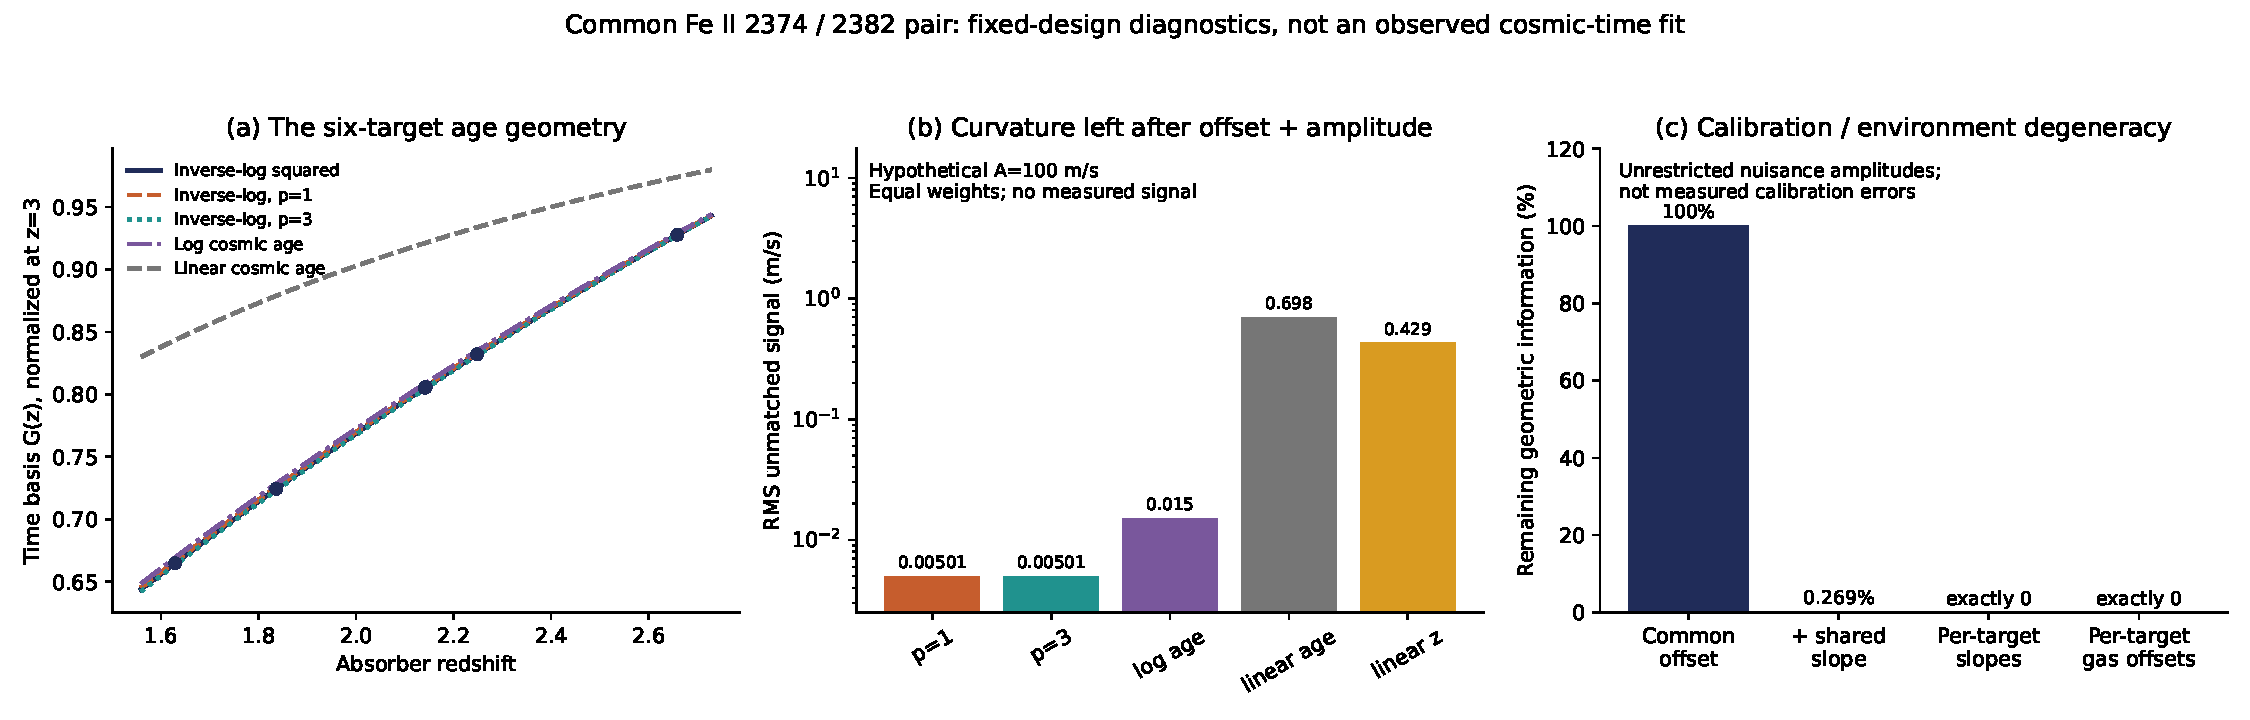
\includegraphics[width=.99\textwidth]{../experiments/highz_feasibility_2026-09-20/results/cross_age/cross_age_identifiability.pdf}
\caption{Fixed-design sensitivity at the six candidate redshifts. The curves and information calculations use no measured line shifts. Free differential offsets for individual absorbers span the age response; more restrictive nuisance assumptions retain conditional information. Competing temporal functions are compared after optimizing their common intercept and amplitude, so raw differences caused only by normalization are removed. All velocity scales in the scenario panels are assumed, not detected.}
\label{fig:age_design}
\end{figure}

The nuisance-space calculation in Fig.~\ref{fig:age_design} illustrates two distinct limitations. Allowing an independently free differential calibration slope for each target gives a full-row-rank nuisance matrix: each slope multiplies a nonzero observed separation of the two transitions. An arbitrary time-amplitude change can then be cancelled exactly. Free target-specific gas or environmental offsets have the same property. This is a statement about identifiability under unrestricted nuisance freedom, not evidence that actual systematics have arbitrary size. A common wavelength zero point cancels between the two lines and cannot produce this degeneracy.

The closeness of this line pair does suppress smooth long-range calibration errors. At the six redshifts its observed separation is approximately $21.83$--$30.38\,\text{\AA}$. Hypothetical velocity-distortion slopes of 50, 200 and $500\,\mathrm{m\,s^{-1}}$ per $1000\,\text{\AA}$ give pair offsets of $1.09$--$1.52$, $4.37$--$6.08$ and $10.92$--$15.19\,\mathrm{m\,s^{-1}}$, respectively. These are propagated scenarios, not adopted empirical priors. If only one slope is shared by all six targets, it leaves $0.269\%$ of the equal-weight age information available with a free intercept alone. However, matching the illustrative $A=100\,\mathrm{m\,s^{-1}}$ age curve actually requires approximately $3077\,\mathrm{m\,s^{-1}}$ per $1000\,\text{\AA}$, with a remaining $0.429\,\mathrm{m\,s^{-1}}$ RMS. Thus a near-degenerate shape cannot be used to claim that modest smooth distortions explain an arbitrarily large effect. Finite independent calibration constraints would restore finite conditional information; short-scale errors and gas-model biases require separate treatment.

Even with those systematics controlled, detecting a trend would not identify its exponent. After re-fitting a common offset and amplitude, $p=1$ and $p=3$ reproduce a $p=2$, $A=100\,\mathrm{m\,s^{-1}}$ scenario to approximately $0.005\,\mathrm{m\,s^{-1}}$ RMS at these six redshifts. An ordinary logarithm of cosmic age differs by $0.015\,\mathrm{m\,s^{-1}}$ RMS, and a linear-age model by $0.698\,\mathrm{m\,s^{-1}}$. These differences arise because a Planck-time reference makes $\ln(t/t_*)$ large compared with its change across this age interval. They scale with the assumed amplitude and are fixed-design model distances, not measured objective differences, detection powers or physical upper bounds.

The pair J053007$-$250329 and J233156$-$090802 is also informative in principle: their rounded catalogue redshifts, 2.141 and 2.143, correspond to an age difference of approximately $2.86\,\mathrm{Myr}$ in this coordinate. The same illustrative age model predicts a difference of only $0.051\,\mathrm{m\,s^{-1}}$. A larger measured difference between such sightlines would test the combined target-dependent effects, provided both descriptors were reliable; it would not uniquely isolate an environmental or instrumental cause. Rounded catalogue redshifts and adopted cosmology do not imply precisely measured ages.

We therefore do not regress the available exploratory offsets into a measured cosmic amplitude. A calibrated cross-age test requires comparable profile constraints, external restrictions on differential systematics, and a specified physical response. The finite set of transitions measures selected energy differences; it does not sample the full symmetry-resolved atomic-level distribution or establish a correspondence to Riemann-zero spacing statistics.


\section{Discussion}
\label{sec:discussion}

\subsection{What a residual relative shift establishes}
The ESPRESSO free-shift extension improves its specified objective, and several controls retain part of that preference. A low absolute quadratic statistic does not erase the matched-model comparison. However, one gas decomposition, fixed atomic inputs and an approximate covariance do not close a systematic-error budget. The result establishes a model discrepancy without identifying a physical-frequency change.

Changing the estimator changes the conditional question. Native exposures and their combined spectrum agree under the same fixed-template estimator; shared photons and template prevent independent confirmation. Removing strong cores changes both possible model inadequacy and displacement information. The local projection quantifies the latter for one direction, without establishing what caused the observed reduction.

The model-construction concerns examined by \citet{Lee2023Models} remain relevant. Opposite-hypothesis starts and saved endpoints expose local minima but do not sample all component structures. Our merged architecture also changes bound centres. Profile searches that find lower objectives are therefore substantive revisions, not merely uncertainty calculations around an established global minimum. Small endpoint changes or successful stopping flags do not certify stationarity.

\subsection{What overlapping orders add}
An actual rest frequency cannot depend on which order records the transition. The retained 2600 contrast therefore directs attention to the observation and its model. Different sampling, masks and weights can interact with a shared imperfect gas template, so the contrast alone cannot isolate a wavelength solution, extraction step or LSF error. Matching coverage addresses one part of this problem.

Non-Gaussian ESPRESSO response is independently established \citep{Schmidt2024LSF}. Our positive kernel changes shape without changing its centroid, yet retains a contrast near $-59\,\mathrm{m\,s^{-1}}$. This rules out removal by the particular fitted family, not by all conventional responses. Sharing a kernel across traces and epochs is especially restrictive. Neither the fit nor its limited transfer performance supplies independently calibrated kernels for the historical science exposures.

The later exposures contain disjoint photons but share the gas template and reduction procedure. Barycentric velocity, detector position and observing period are also correlated. Absence of a simple univariate trend does not exclude nonlinear effects, and a trend among correlated predictors would not establish causation. Exposure-level forward modelling with external calibration addresses this remaining gap.

\subsection{From more spectra to an identifiable cross-epoch test}
Catalogue coverage, a detected multiplet and a satisfactory local fit are different readiness levels. Boundaries, truncated structure and initialization dependence cannot be discarded to obtain one regression point per absorber. Moreover, an $H_0$-adequacy filter could exclude genuinely shifted systems; the filtered diagnostic sample is not an unbiased population test of constant frequencies.

Keeping the 2382/2374 pair fixes the observable across redshifts. Unrestricted target-specific differential offsets nevertheless span its age response. This algebraic result does not imply arbitrary physical systematic amplitudes: the close pair suppresses smooth long-range distortions, and the finite slope scenarios in Sec.~\ref{sec:identifiability} produce much smaller offsets than a widely separated pair would. Independently justified bounds restore conditional information. Near-collinearity alone cannot show that modest distortions explain an arbitrarily large effect.

A shared laboratory-ratio error contributes an intercept, whereas target-specific differential terms need not. Even after controlling them, detecting a trend would not select its exponent. At these six ages, the normalized $p=1,2,3$ schedules are nearly identical after adjusting intercept and amplitude. Their small shape distances are fixed-design calculations, not measured trend evidence or physical amplitude bounds.

The inverse-logarithmic family is motivated by the author's numerical non-autonomous-map study associated with Riemann-zero data \citep{Wang2026Spectral}. It supplies no atomic Hamiltonian or Fe\,II response. An added uncertainty \emph{standard deviation} is not a deterministic level displacement: stochastic models require correlation and line-shape calculations, while drift models require level-dependent coefficients. The present diagnostics test prerequisites without asserting that physical connection.

\subsection{A prospective prediction test}
\label{sec:prospective}
A prospective extension would freeze an age-dependent prediction before examining independent validation sightlines. Keeping the same Fe\,II 2382/2374 descriptor, illustrative groups at $z=1,1.5,2$ sample cosmic ages of approximately $5.85$, $4.26$ and $3.27\,\mathrm{Gyr}$ in the adopted coordinate. Under the fixed inverse-log-square schedule, development anchors at the low and high redshifts predict
\begin{equation}
 D(1.5)_{\rm pred}=0.45756\,D_{\rm dev}(1)
                   +0.54244\,D_{\rm dev}(2).
 \label{eq:prospective_prediction}
\end{equation}
For an illustrative endpoint difference of $100\,\mathrm{m\,s^{-1}}$, the intermediate difference is $54.24\,\mathrm{m\,s^{-1}}$; neither amplitude is measured or derived from an atomic theory here. New endpoint sightlines must independently reproduce a nonzero contrast, because a constant also satisfies Eq.~\ref{eq:prospective_prediction}. Instrument, observing-condition and near-equal-redshift controls would test alternative explanations. A sufficiently precise disagreement would reject the frozen nonzero forecast; inconclusive precision would not validate it. Such a deterministic mean response is an additional hypothesis beyond an uncertainty floor. Appendix~\ref{app:prediction} specifies sample separation, covariance, failure rules, conditional power and current instrument constraints. This is a proposed protocol, with no registered prediction, selected observing programme or new observations. It does not resolve the near-degeneracy among inverse-logarithmic exponents.

\section{Conclusions}
\label{sec:conclusions}
The public observations support reproducible sensitivity tests: matched gas-model comparisons, continuum covariance controls, fixed-mask information calculations, native-order contrasts and additional archive profiles. They expose conditional inconsistencies and numerical/model dependence, while separating available spectra from calibrated frequency measurements.

A confirmation programme needs independent differential calibration, broader gas/covariance assessment, a common transition pair and selection fixed before examining shifts. Inadequate fits must remain visible. With a specified physical response, such data could constrain a time-dependent amplitude or test whether a reproduced residual follows an age law. The current study establishes neither a calibrated astrophysical frequency change nor a preferred aging exponent.


\section*{Data and code availability}
The analysis code, source manifests, processed arrays, numerical endpoints and validation reports accompany this manuscript in the \texttt{riemann\_clock} project. Public ESPRESSO products and atomic/component inputs are provided by the \citet{Murphy2022ESPRESSO} data release, archived at \url{https://doi.org/10.5281/zenodo.5512490}. The UVES spectra and source catalogues are from SQUAD DR1 \citep{Murphy2019SQUAD}. Source URLs, repository revisions, file sizes and hashes are recorded in the accompanying manifests; third-party files retain their original provenance and applicable terms. The accompanying records distinguish historical observations, products reprocessed later, and calculations performed in this study. The availability of a paper describing another reduction is not treated as acquisition of its science arrays or response matrices.

\section*{Author and assistance statement}
Liang Wang supplied the research questions and source projects. AI assistance was used in literature retrieval, source auditing, code preparation, numerical checking and manuscript drafting. Responsibility for the scientific claims and submitted version remains with the author. No institutional affiliation, funding source, competing-interest declaration or external peer-review status is inferred in this draft.

\appendix
\section{Prospective relative-frequency prediction protocol}
\label{app:prediction}

\subsection{Observable, physical assumption, and fixed prediction}
\label{app:prediction_model}

This prospective design tests the apparent relative frequency of two Fe\,II
transitions, not a complete energy-level distribution.  The original
Riemann-motivated hypothesis concerns an additional uncertainty \emph{standard
deviation} proportional to $\ln^{-2}(t/t_*)$; it does not derive a mean line-centre
drift.  We explicitly add a universal deterministic mean response.  Testing
stochastic broadening instead would require independent atomic-response and
temporal/spatial-correlation models, and a separate protocol.  Failure of one
endpoint cannot be reinterpreted as success of the other.

The primary descriptor is fixed to
\begin{equation}
 D(z)=v_{2382}-v_{2374},\qquad Y_{\rm app}=-D/c.
 \label{app:descriptor}
\end{equation}
A common logarithmic-velocity zero point cancels, whereas differential
calibration, gas, isotope, and environmental effects remain.  A uniform
fractional rescaling of all transition frequencies can be absorbed into
redshift and is outside this test's sensitivity.

The age coordinate is a fixed flat matter--$\Lambda$ model with
$H_0=67.4\ {\rm km\,s^{-1}\,Mpc^{-1}}$, $\Omega_m=0.315$, and no radiation.
Set $t_0=t(0)$ and $t_*=5.391247\times10^{-44}\ {\rm s}$, using consistent time
units inside dimensionless logarithms.  Define
\begin{align}
 f_p(t)&=\left[\frac{\ln(t_0/t_*)}{\ln(t/t_*)}\right]^p-1,
 \label{app:time_function}\\
 H_p(z)&=\frac{f_p[t(z)]-f_p[t(1)]}{f_p[t(2)]-f_p[t(1)]},
 &D(z)&=b+B H_2(z).
 \label{app:endpoint_model}
\end{align}
Here $b=D(1)$ and $B=D(2)-D(1)$, in velocity units.  This normalization differs
from $D=b_{\rm old}+A G_2(z)$ with $G_p(z)=f_p[t(z)]/f_p[t(3)]$:
$B=0.312753948A$, with a corresponding intercept change.  Neither $B$ nor its
sign is currently predicted by the underlying hypothesis or measured by this
design calculation.  The cosmology, $t_*$, and primary exponent $p=2$ must not
be tuned using confirmation data.

At the illustrative design centres $z=(1,1.5,2)$, ages are
$(5.845622,4.264167,3.273357)$ Gyr and $H_2=(0,r,1)$, with
$r=0.542436444$.  Development estimates of the two endpoints therefore predict
a previously unexamined middle group:
\begin{equation}
 D(1.5)_{\rm pred}=0.457563556D(1)+0.542436444D(2).
 \label{app:midpoint_prediction}
\end{equation}
The hypothetical choice $B=100\ {\rm m\,s^{-1}}$ gives a middle-minus-low
contrast of $54.2436\ {\rm m\,s^{-1}}$; these are illustrative values, not
observations or theoretical amplitudes.  Actual predictions use each target's
redshift.  Group weights and averages of $H_2$ are frozen; applying $H_2$ to a
broad bin's mean redshift is not equivalent.

\subsection{Development, freezing, and independent confirmation}
\label{app:prediction_samples}

The existing seventeen ESPRESSO exposures and six archive candidates are
development material.  Future calibrated low- and high-redshift development
sightlines determine $b,B$, nuisance treatment, and predictive uncertainty.
An unconstrained or near-zero amplitude cannot yield a sharp nonzero
forecast.  Before accessing confirmation shifts, a public timestamped protocol
must fix target identities, selection and exclusion rules, code and data
versions, the fitted prediction and covariance, primary statistic and
threshold, bias budget, scientifically relevant $B_{\min}$, equivalence
tolerance, and stopping rules.  Current file hashes support reproducibility;
they do not constitute public preregistration.

Confirmation requires new independent sightlines in all three redshift
groups.  New endpoint targets replicate the nonzero contrast; a new midpoint
with old endpoints alone cannot do so.  Multiple absorbers on one sightline
share calibration uncertainty.  A provisional organization of four
development sightlines per endpoint and eight confirmation sightlines per
group totals 32, but establishes neither target availability nor adequate
power.  Final sample size follows blinded pilot precision and $B_{\min}$,
with at most one prespecified update using blinded quality/noise information,
never repeated additions until significance.

Zero- and nonzero-signal injections must cover gas architecture, response,
pixel covariance, optimization, and interval coverage.  Poor fit by a
constant-frequency model alone must not exclude a potentially shifted target;
failures follow frozen rules and remain reported.  Each redshift group needs
an independent-instrument subset, interleaved seasons/nights, and matched
absorption depth, width, saturation, and measurable environment.  Barycentric
velocity, trace, and valid overlapping-order controls test instrumental
stability.  Reobserving one absorber years later supplies no gigayear age
baseline; nearby-redshift independent sightlines instead constrain target
scatter.

\subsection{Prediction covariance and conventional-bias bounds}
\label{app:prediction_covariance}

For $\mathbf y=(D_L,D_M,D_H)^{\mathsf T}$, define
\begin{equation}
 C=\mathbf w^{\mathsf T}\mathbf y,
 \qquad\mathbf w=(-(1-r),1,-r)^{\mathsf T},
 \qquad\operatorname{Var}(C)=\mathbf w^{\mathsf T}\Sigma\mathbf w.
 \label{app:closure}
\end{equation}
For the frozen forecast, $L,H$ are development anchors and $M$ is new
confirmation data.  Closure among three new confirmation groups is an
additional shape diagnostic.  Crucially, $B=0$ also gives $C=0$: closure
cannot establish variation without independent nonzero endpoint replication.

The joint $\Sigma$ includes development uncertainty, validation errors, shared
laboratory references, calibration, sightlines, and trained models, including
cross-covariances.  Independent equal group errors $\sigma_g$ give
$\sigma_C=1.226214\sigma_g$ only as a special case.  A common laboratory
pair-zero covariance $\sigma_{\rm lab}^2\mathbf1\mathbf1^{\mathsf T}$ cancels
because $\mathbf w^{\mathsf T}\mathbf1=0$; wavelength distortions and
age-correlated environmental biases generally do not.

For arbitrary target redshifts, let $X=(1,H_2)$, with development and
validation subscripts $T,V$.  Fixed-covariance generalized least squares gives
\begin{align}
 M&=(X_T^{\mathsf T}\Sigma_{TT}^{-1}X_T)^{-1}
       X_T^{\mathsf T}\Sigma_{TT}^{-1},
 &\widehat{\boldsymbol\theta}&=M\mathbf y_T,
 \label{app:development_estimator}\\
 \mathbf e_V&=\mathbf y_V-X_VM\mathbf y_T.
 \label{app:validation_residual}
\end{align}
The predictive covariance is
\begin{equation}
 \begin{split}
 \Sigma_e={}&\Sigma_{VV}
 +X_VM\Sigma_{TT}M^{\mathsf T}X_V^{\mathsf T}\\
 &-\Sigma_{VT}M^{\mathsf T}X_V^{\mathsf T}
 -X_VM\Sigma_{TV}.
 \end{split}
 \label{app:full_prediction_covariance}
\end{equation}
Estimated covariance, model selection, or active bounds require full
injection-based coverage calibration, not an automatic exact $\chi^2$ claim.
Unknown bounded biases $|d_i|\leq\epsilon_i$ instead allow a closure bias up to
$\sum_i|w_i|\epsilon_i$, or $2\epsilon$ for equal bounds.  Structured biases
require maximization over their allowed set.  Such bounds must not be
silently converted into independent zero-mean Gaussian errors.

\subsection{Conditional power and instrument requirements}
\label{app:prediction_power}

Table~\ref{app:power_table} assumes eight confirmation targets per endpoint,
independent single-target random error $\sigma$, and known zero-mean Gaussian
group offsets of dispersion $\tau$, independent between groups.  Then
\begin{equation}
 \sigma_\Delta^2=2(\sigma^2/8+\tau^2).
 \label{app:power_variance}
\end{equation}
Correlated group offsets require the additional $-2\operatorname{Cov}$ term.
The two-sided $\alpha=0.01$ planning threshold neither calibrates unknown
systematics nor constitutes a discovery standard.

\begin{table}[tbp]
 \centering
 \caption{Hypothetical endpoint power for $|B|=100\ {\rm m\,s^{-1}}$ and
 eight targets per endpoint.  All velocity columns are in
 ${\rm m\,s^{-1}}$.  $|B|_{90\%}$ is the effect required for 90\% power under
 the stated known-Gaussian assumptions; no row represents measured performance.}
 \label{app:power_table}
 \begin{tabular}{rrrrr}
 \toprule
 $\sigma$ & $\tau$ & $\sigma_\Delta$ & Power & $|B|_{90\%}$\\
 \midrule
 50 & 10 & 28.72 & 81.7\% & 110.8\\
 100 & 20 & 57.45 & 20.2\% & 221.6\\
 200 & 30 & 108.63 & 4.9\% & 419.0\\
 \bottomrule
 \end{tabular}
\end{table}

The first scenario needs eleven targets per endpoint for 90\% power at
$|B|=100\ {\rm m\,s^{-1}}$, before development, midpoint, and replication
resources.  The other two cannot reach 90\% by increasing target numbers
alone because their group-error floors remain.

ESPRESSO covers 380--788 nm, with median HR resolving power approximately
140,000 \citep{ESOESPRESSO2026}.  The P117 manual places the current laser
frequency comb's blue end near 450 nm \citep{ESOESPRESSOManualP117}.
The proposed pair lies near 475/477, 594/596, and 712/715 nm; the high-redshift
windows require prior water-vapour screening.  The $z\simeq0.7$ pair is below
the current comb range and is excluded from this primary design.  HR plus
sky should be evaluated for faint quasars: the B fibre records sky or
Fabry--P\'erot, not both.  LFC/ThAr calibration is daytime operation, so
night-time comb exposures immediately bracketing science cannot be promised
\citep{ESOESPRESSOManualP117}.  Actual calibration chains and independent
drift/response constraints must be preserved; a science-fitted response is
not independent calibration.  Target-specific exposure-time calculations,
clean windows, and injection recovery precede any observing-hours claim.

\begin{figure}[tbp]
 \centering
 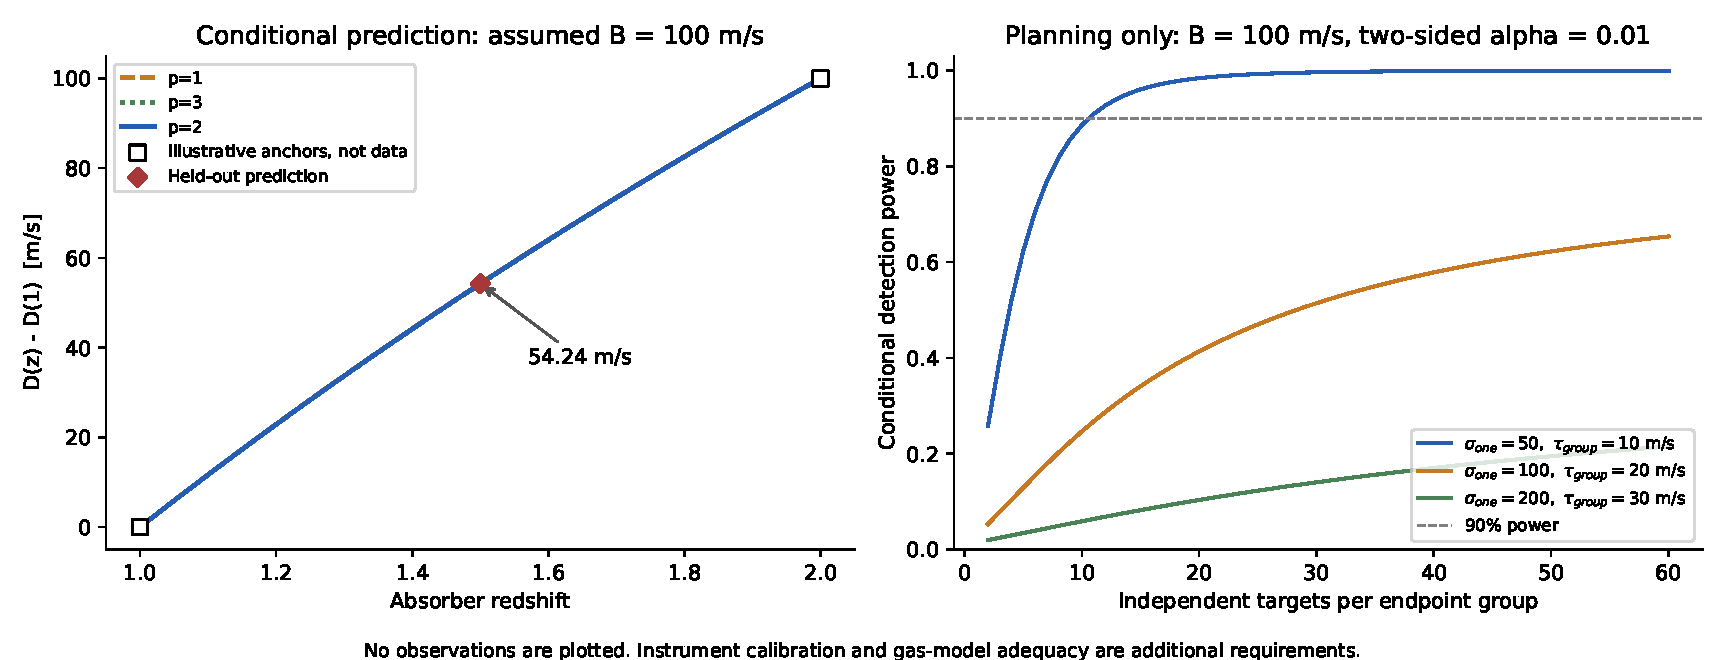
\includegraphics[width=0.98\textwidth,height=0.43\textheight,keepaspectratio]
 {../experiments/prediction_test_2026-09-21/figures/prediction_design.pdf}
 \caption{Conditional prediction geometry and hypothetical power calculations.
 There are no observed data points.  The displayed
 $B=100\ {\rm m\,s^{-1}}$ is illustrative; power assumes the stated Gaussian
 group-error floors and is not target-specific instrument performance.}
 \label{app:prediction_figure}
\end{figure}

\subsection{Failure criteria and scope of future conclusions}
\label{app:prediction_outcomes}

A replicated nonzero endpoint contrast, a sufficiently narrow interval
compatible with the frozen midpoint prediction, and successful conventional
controls would support the tested mean-response model over this sample range.
Adequate precision excluding its frozen direction or amplitude constitutes
failure of that prediction.  Midpoint disagreement implicates the shape,
universality, or measurement model; instrument-dependent shifts fail physical
attribution, and dominant same-age scatter requires environmental/gas checks.
Wide intervals covering both zero and the forecast are inconclusive.

Because $B=0$ remains allowed, a null result cannot exclude the whole
free-amplitude family.  A researcher-selected $B_{\min}$ is a relevance
threshold, not a theoretical lower bound.  Furthermore, after matching the
same endpoints at $B=100\ {\rm m\,s^{-1}}$, $p=1$ and $p=3$ alter the midpoint
by only approximately $+0.0517$ and $-0.0517\ {\rm m\,s^{-1}}$.  A detected
trend would therefore not identify $p=2$ or establish a Riemann origin.

As of 21 September 2026 this protocol is unregistered, with no frozen
amplitude, final qualified target list, allocated telescope time, or new
observations.  Existing instruments permit preparatory work; neither a
ten-year discovery nor an achievable precision is promised before target and
calibration qualification.


\bibliographystyle{plainnat}
\bibliography{references}
\end{document}
